\begin{figure}[htb]
\centering
\begin{tikzpicture}
%\draw[help lines,step=1] (-4,-4) grid (8,4);
\draw [rectangle, black, draw, rounded corners=2ex,line width=0.25ex] (1.6,-0.5) rectangle (3.4,1.5);

\draw (1,0) -- (3,0);
\draw (2,1) -- (3,1) -- (2,0) -- (3,0) -- cycle;
\node [fill=gray!30, radius=1ex, draw, circle, inner sep=2pt] at (2,1) {$e$};
\node [fill=gray!30, radius=1ex, draw, circle, inner sep=2pt] at (3,1) {$f$};
\node [fill=gray!30, radius=1ex, draw, circle, inner sep=2pt] at (2,0) {$g$};
\node [fill=gray!30, radius=1ex, draw, circle, inner sep=2pt] at (2,0) {$g$};
\node [fill=gray!30, radius=1ex, draw, circle, inner sep=2pt] at (3,0) {$h$};
\draw (0,1) -- (1,1);
\draw (1,1) -- (1,0);
\draw (1,0) -- (1,1);
\draw (1,1) -- (0,0);
\node [fill=gray!30, radius=1ex, draw, circle, inner sep=2pt] at (0,1) {$a$};
\node [fill=gray!30, radius=1ex, draw, circle, inner sep=2pt] at (1,1) {$b$};
\node [fill=gray!30, radius=1ex, draw, circle, inner sep=2pt] at (0,0) {$c$};
\node [fill=gray!30, radius=1ex, draw, circle, inner sep=2pt] at (1,0) {$d$};
\node at (2.5,1.75) {$\mathcal{G}$};
\node at (0.5,1.75) {{\color{red}$G-\mathcal{G}$}};
\draw [rectangle, red, draw, rounded corners=2ex,line width=0.25ex] (-0.4,-0.5) rectangle (1.4,1.5);
\node [] at (5.5,1) {$\Pr(\mathcal{G}) = \dfrac{\binom{6}{4} \binom{28-4}{10-6}}{\binom{28}{10}}$};
\node [] at (6.0,0) {$\approx 0.0121$};

\node [] at (9.5,1) {$m_c=4,p_c=6,n_c=4$};
\node [] at (9.5,0) {$p=28,m=10,n=8$};
\end{tikzpicture}
\caption{Probability for the subgraph $\mathcal{G}=(\mathcal{V},\mathcal{E})$ where $\mathcal{V}=\{e,f,g,h\}$ and $\mathcal{E}=\{(e,f),(f,g),(g,h),(e,h)\}$ to be randomly drawn from the graph $G$.}
\label{fig:subgraphconditionalprobability}
\end{figure}